\chapter{Theory}
\label{cha:theory}

% The main purpose of this chapter is to make it obvious for
% the reader that the report authors have made an effort to read
% up on related research and other information of relevance for
% the research questions. It is a question of trust. Can I as a
% reader rely on what the authors are saying? If it is obvious
% that the authors know the topic area well and clearly present
% their lessons learned, it raises the perceived quality of the
% entire report.
% 
% After having read the theory chapter it shall be obvious for
% the reader that the research questions are both well
% formulated and relevant.
% 
% The chapter must contain theory of use for the intended
% study, both in terms of technique and method. If a final thesis
% project is about the development of a new search engine for
% a certain application domain, the theory must bring up related
% work on search algorithms and related techniques, but also
% methods for evaluating search engines, including
% performance measures such as precision, accuracy and
% recall.
% 
% The chapter shall be structured thematically, not per author.
% A good approach to making a review of scientific literature
% is to use \emph{Google Scholar} (which also has the useful function
% \emph{Cite}). By iterating between searching for articles and reading
% abstracts to find new terms to guide further searches, it is
% fairly straight forward to locate good and relevant
% information, such as \cite{test}.
% 
% Having found a relevant article one can use the function for
% viewing other articles that have cited this particular article,
% and also go through the article’s own reference list. Among
% these articles on can often find other interesting articles and
% thus proceed further.
% 
% It can also be a good idea to consider which sources seem
% most relevant for the problem area at hand. Are there any
% special conference or journal that often occurs one can search
% in more detail in lists of published articles from these venues
% in particular. One can also search for the web sites of
% important authors and investigate what they have published
% in general.
% 
% This chapter is called either \emph{Theory, Related Work}, or
% \emph{Related Research}. Check with your supervisor.

This chapter introduces relevant theory and related work.
Section ~\ref{sec:activevision} gives some background on active vision.
Section ~\ref{sec:visualsearch} describes the problem of visual searching for targets.


% describe how animal vision translates to camera vision?
% animals have a large field of view, but also require foveated vision: processing is expensive.
% computers do not naturally have this constraint and most CV algorithms do not use foveated vision
% (although visual attention models exist)

\section{Artificial Neural Networks}

An artificial neural network (ANN) is a type of universal function approximator.

% https://davidstutz.de/illustrating-convolutional-neural-networks-in-latex-with-tikz/

\subsection{Multi-layer Perceptron}

\subsection{Long Short-Term Memory}

% https://colah.github.io/posts/2015-08-Understanding-LSTMs/

\subsection{Convolutional Neural Network}

% https://viso.ai/deep-learning/mask-r-cnn/#:~:text=Mask%20R%2DCNN%20is%20a,segmentation%20mask%20for%20each%20instance.

\section{Reinforcement Learning}

Reinforcement learning (RL) is a subfield of machine learning concerned with learning from interaction how to achieve a goal.

\subsection{Partially Observable Markov Decision Process}

The problem of learning from interaction to achieve some goal is often framed as a (finite) Markov decision process (MDP).
In this work, we consider a partially observable Markov decision process (POMDP).
Formally, a POMDP is defined as a 7-tuple \(\langle \mathcal{S}, \mathcal{A}, \mathcal{O}, \mathcal{P}, \mathcal{R}, \mathcal{Z}, \gamma \rangle\), where

\begin{itemize}
    \item \(\mathcal{S}\) is a finite set of states,
    \item \(\mathcal{A}\) is a finite set of actions,
    \item \(\mathcal{O}\) is a finite set of observations,
    \item \(\mathcal{P}\) is a set of conditional transition probabilities between states,
    \item \(\mathcal{R}\) is a reward function,
    \item \(\mathcal{Z}\) is an observation function, and
    \item \(\gamma \in [0, 1]\) is a discount factor.
\end{itemize}

A learning \textit{agent} interacts continually with its \textit{environment}.
At each discrete time step, the environment is in some \textit{state} \(s \in \mathcal{S}\).
The agent picks an \textit{action} \(a \in \mathcal{A}\) to take.
This puts the environment in state \(s^\prime\) with probability \(\mathcal{P}(s^\prime | s, a)\).
The agent receives an \textit{observation} \(o \in \mathcal{O}\) with probability \(\mathcal{Z}(o | s^\prime, a)\).
It also receives a \textit{reward} \(r\) given by \(\mathcal{R}(s, a)\).

The agent and environment interact over a sequence of discrete time steps \(t = 0, 1, \dots, T\), giving rise to a \textit{trajectory} of length \(T\).
The goal of the agent is to maximize the expected \textit{discounted return} \(G_t \doteq \sum_{k=t+1}^{T}\gamma^{k-t-1}r_k\), where \(\gamma\) represents the uncertainty of the environment.  
Figure \ref{fig:pomdp} illustrates this process.

\begin{figure}
    \centering
    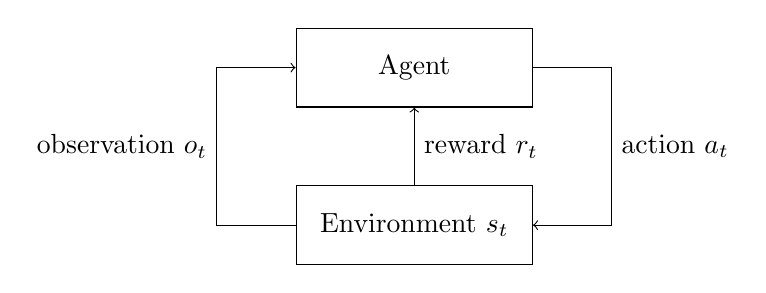
\begin{tikzpicture}[node distance=2cm]
    \tikzstyle{block} = [rectangle,minimum width=3cm,minimum height=1cm,text centered,draw=black,fill=white]
    \node (agent)[block]{Agent};
    \node (environment)[block,below of=agent]{Environment \(s_t\)};
    \draw [->] (agent.east) -- ++(1cm,0) -- node [anchor=west]{action \(a_t\)} ++(0,-2cm) -- (environment.east);
    \draw [->] (environment.north) -- node [anchor=west]{reward \(r_t\)} (agent.south);
    \draw [->] (environment.west) -- ++(-1cm,0) -- node [anchor=east]{observation \(o_t\)} ++(0,+2cm) -- (agent.west);
\end{tikzpicture}
    \label{fig:pomdp}
    \caption{Partially observable Markov decision process.}
\end{figure}

Since the agent receives partial observations of the environment's state, it has to act under uncertainty.
Planning in a POMDP is undecidable, and solving them is often computationally intractable.
Approximate solutions are more common.
% belief state

\subsection{Policies and Value Functions}

Most RL algorithms estimate both a \textit{value function} that tells the agent how good it is to be in a given state.


\section{Related Work}

\subsection{Deep Reinforcement Learning}

% Mnih et al., Atari, DQN

A long-standing challenge in RL is to learn good policies from high-dimensional sensory inputs like vision.
Mnih et al. (2013)~\cite{mnih_atari_2013} address this by combining deep learning with RL.
A CNN is trained to estimate the 
% deep learning
% experience replay
% value iteration
% deep Q-learning

Hausknecht and Stone (2017)~\cite{hausknecht_stone_2017} investigates the effects of adding recurrency to a DQN in order to tackle POMDPs.
A LSTM is added after the initial 

\subsection{Local Search}
% Artificial Intelligence - A modern approach
% Page 134
% Should cover belief states?
% ~\cite{russell_artificial_2021}
% https://en.wikipedia.org/wiki/Tabu_search
% tabu search is mentioned in russel
% could be interesting as inspiration for reward function
% and also observation space
% bring in "learning to optimize" here

% an annealed step size could be interesting...
% more general and there are certainly parallells to other areas.

% local search
% https://en.wikipedia.org/wiki/Local_search_(optimization)
% https://en.wikipedia.org/wiki/Guided_Local_Search

% "learning local search"
% "learning to optimize"

% Reinforcement Learning for Local Search

% Learning Neural Network Policies with Guided Policy Search under Unknown Dynamics
% Levine et al. seems like it could be useful

% we could draw inspiration from multiple local search approaches

% it is essentially a combinatorial optimization problem (I think)

%Schuurman & Southey propose three measures of effectiveness for local search (depth, mobility, and coverage):[2]
%
%    depth: the cost of the current (best) solution;
%    mobility: the ability to rapidly move to different areas of the search space (whilst keeping the cost low);
%    coverage: how systematically the search covers the search space, the maximum distance between any unexplored assignment and all visited assignments.


\subsection{Active Vision}
\label{sec:activevision}

% Marr?

Much of past and present research in machine perception involves a passive observer.
Images are passively sampled and perceived.
Animal perception, however, is active.
We do not only see things, but look for them.
One might ask why this is the case, if there is any advantage that an active observer has over a passive one.
Aloimonos and Weiss (1988)~\cite{aloimonos_active_1988} introduce the paradigm called \textit{active vision}, and prove that an active observer can solve several basic vision problems in a more efficient way than a passive one.

Bajcsy (1988)~\cite{bajcsy_1988} defines active vision, and perception in general, as a problem of intelligent data acquisition.
An active observer needs to define and measure parameters and errors from its scene and feed then back to control the data acquisition process.
Bajscy states that one of the difficulties of this problem is that they are scene and context dependent.
A thorough understanding of the data acquisition parameters and the goal of the visual processing is needed.
One view lacks information that may be present with multiple views.
Multiple views also add the time dimension into the problem.

In a re-visitation of active perception, Bajcsy, Aloimonos and Tsotsos (2018)~\cite{bajcsy_aloimonos_tsotsos_2018} stress that despite recent successes in robotics, artificial intelligence and computer vision, an intelligent agent must include active perception:

\begin{quote}
    An agent is an active perceiver if it knows why it wishes to sense, and then chooses what to perceive, and determines how, when and where to achieve that perception
\end{quote}~\cite{bajcsy_aloimonos_tsotsos_2018}

% see conclusion in that paper:
% - mirror neurons, same system responsible for generating and interpreting actions at a high level 

\subsection{Visual Search}
\label{sec:visualsearch}

The perceptual task of searching for something in a visual environment is usually referred to as \textit{visual search}.
The searched object or feature is the \textit{target}, and the other objects or features in the environment are the \textit{distractors}.
This task has been studied extensively in psychology and neuroscience.

Wolfe (2021)~\cite{wolfe_guided_2021} describes a model of visual search

% general things
% - foveated vision
% - covert and overt attention
% ...

Eckstein (2011)~\cite{eckstein_visual_2011} reviews efforts from various subfields and identifies a set of mechanisms used to achieve efficient visual search.
Knowledge about the target, distractor, background statistical properties, location probabilities, contextual cues, rewards and target prevalence are all identified as useful.
This is motivated with evidence from psychology as well as neural correlates.

Visual search is not always instant, and can in fact often be slow.
This is in part due to processing: our visual system cannot process the entire visual field and 

% saliency, center-surround organization
% covert attention and eye movement

Wolfe and Horowitz (2017)~\cite{wolfe_horowitz_2017} identify and measure a set of factors that guide attention in visual search.
One of these is bottom-up guidance, in which some visual properties of the scene draw more attention than others.
Another is top-down guidance, which is user driven and directed to objects with known features of desired targets.
Scene guidance is also identified, in which attributes of the scene guide attention to areas likely to contain targets. 

These works ground the task considered in this project in psychology.

% can we build a system that exhibits all of these?

\subsection{Object Detection}

% active object detection

A similar problem can be found in the computer vision literature under \textit{object detection}.
The goal of object detection is to, given an input image, detect instances of semantic objects in it.
This includes assigning a bounding box to the objects, and classifying the object.
The input image is usually passively sampled, and the whole scene is visible at once.

Caicedo and Lazebnik (2015)~\cite{caicedo_active_2015} propose to use deep reinforcement learning for active object localization in images where the object to be localized is fully visible.
An agent is trained to successively improve a bounding box using translating and scaling transformations.
They use a reward signal that is proportional to how well the current box covers the target object.
An action that improves the region is rewarded with +1, and -1 otherwise.
Without this quantization, the difference was small enough to confuse the agent.
Binary rewards communicate more clearly which transformations keep the object inside the box and which take the box away from the target.
When there is no action that improves the bounding box, the agent may select a trigger action (which would be the only action that does not give a negative reward) which resets the box.
This way the agent may select additional bounding boxes.
Each trigger modifies the environment by marking it so that the agent may learn to not select the same region twice.
This is referred to as an inhibition-of-return mechanism, and is widely used in visual attention models~\cite{[16] in caicedo_active_2015}.
This method has a few shortcomings for the problem considered in this project.
The object may not be visible in the initial frame so the agent cannot act in the same way. 

A separate field is active object search, which is perhaps most closely related to the problem we consider in this work.
In active object search, % explain
% difference is tht this is the first deep dive into these particular aspects
% write about the work that uses object co-occurences though
% we should stress that we do not explicitly model the environment guidance, but are rather interested in whether it can be learned efficiently by the system

% Visual Navigation is another thing to call it...

% 

A similar work by Ghesu et al. (2016)~\cite{ghesu_artificial_2016} present an agent for anatomical landmark detection trained with DRL.
Different from \cite{caicedo_active_2015} is that the entire scene is not visible at once.
The agent sees a limited region of interest in an image, with its center representing the current position of the agent.
The actions available to the agent translate the view up, down, left and aright.
A reward is given to the agent that is equal to the supervised relative distance-change to the landmark after each action.
Three datasets of 891 anatomical images are used.
The agent starts at random positions in the image close to the target landmark and is tasked with moving to the target location.
While achieving strong results (90\% success rate), the scenes and targets are all drawn from a distribution with low variance.
Most real-world search tasks exhibit larger variance than anatomical images of the human body.

Zhu et al. (2016)~\cite{zhu_target_driven_2016} create a model for target-driven visual navigation in indooor scenes with DRL.
An observer is given a partial image of its scene as well as an image of the target object, and is tasked with navigating to the object n the scene with a minimal number of steps.
The agent moves forwards, backwards, and turns left and right at constant step lengths.
They use a reward signal with a small time penalty to incentivize task completion in few steps.
They compare their approach to random walk and the shortest path and achieve promising results.
This setup is quite similar to the one considered in this report, but the authors make a few assumptions that we do not.
They a set of 32 scenes, each of which contain a fixed number of object instances.
They focus on learning spatial relationships between objects in these specific scenes, and have scene-specific layers to achieve this.
Thus, while they show that they can adapt a trained network to a new scene, their approach is unable to zero-shot generalize to new scenes.

A similar work by Ye et al. (2018)~\cite{ye_active_2018} integrates an object recognition module with a deep reinforcement learning based visual navigation module.
They experiment with a set of reward functions and find that constant time penalizing rewards can be problematic and lead to slow convergence.
Their experiments make the same assumptions as \cite{zhu_target_driven} - the scenes and targets used during testing have all been seen during training.


% CT scan material: there is way less variance, otherwise similar. Big difference is that we look at more variance in many aspects?

% CV material: different in that the object is assumed to be visible


\subsection{Visual Attention}

% this article is very good!
% note: reinforcement learning part, soft and hard attention
% https://shairozsohail.medium.com/a-survey-of-visual-attention-mechanisms-in-deep-learning-1043eb25f343

\subsection{Point Navigation}

% https://aihabitat.org/challenge/2020/#task-1-pointnav

\subsection{Object Navigation}

% https://aihabitat.org/challenge/2020/#task-2-objectnav
% https://arxiv.org/pdf/1709.06158.pdf

\subsection{Semantic Navigation}

% https://arxiv.org/pdf/2007.00643.pdf
% proposes a semantic map which is apparently very similar to my proposed method...
% "explicit episodic (semantic) memory"


\subsection{Exploration and Exploitation Trade-off}

% The thesis could also be called Efficient Exploration

% Go into motivation if we use this

% Custom rewards are often needed
% intrinsic?

\subsection{Generalization in Deep Reinforcement Learning}

% reality is dynamic
% agents need to be robust to variation
% capability to transfer and adapt to unseen but similar environments
% most current research works on benchmarks that do not test this (MuJoCo, Arcade learning environment)

% refer to survey
% specifically IID (train_dist = test_dist) and OOD environments (train_dist != test_dist)

% how do they handle training and test set?

Kobbe et al. (2020)~\cite{} study generalization in RL. They introduce a benchmark of procedurally generated i.i.d. environments, and find that this is essential to 




% Could argue that previous works do not clearly show that desireable behaviour is exhibited
% Simpler environments would be better for this, where you can "isolate" more. 